\documentclass[14pt]{book}
\usepackage{array}
\usepackage{amsmath}
\usepackage{amsfonts}
\usepackage{math}
\usepackage{graphicx}
\usepackage{rsfs}
\usepackage{amssymb}
\usepackage{multicol}
\usepackage{caption}
\usepackage{subcaption}
\textwidth=31.9pc
\textheight=46.5pc
\oddsidemargin=1pc
\evensidemargin=1pc
\headsep=15pt
%\headheight=.2cm
\topmargin=.6cm
\parindent=1.7pc
\parskip=0pt


\setcounter{page}{1}
\begin{document}
%\pagestyle{fancy}
\renewcommand{\baselinestretch}{1.2}
%\lhead[\fancyplain{} \leftmark]{}
%\chead[]{}
%\rhead[]{\fancyplain{}\rightmark}
%\cfoot{}
%\headrulewidth=0pt
\markright{
%\hbox{\footnotesize\rm Statistica Sinica
%{\footnotesize\bf ??}(200?), 000-000}\hfill
}
\markboth{\hfill{\footnotesize\rm FIRSTNAME1 LASTNAME1 AND FIRSTNAME2 LASTNAME2
}\hfill}
{\hfill {\footnotesize\rm FILL IN A SHORT RUNNING TITLE} \hfill}
\renewcommand{\thefootnote}{}
$\ $\par
\fontsize{10.95}{14pt plus.8pt minus .6pt}\selectfont
\vspace{0.8pc}
\centerline{\large\bf Dirichlet Distribution And Hyperspectral Imaging Demixing}
\vspace{2pt}
\centerline{\large\bf }
%\vspace{.4cm}
%\centerline{Author(s)}
%\vspace{.4cm}
%\centerline{\it Affiliation(s)}
\vspace{.55cm}
\fontsize{9}{11.5pt plus.8pt minus .6pt}\selectfont

\vspace{9pt}




\fontsize{10.95}{14pt plus.8pt minus .6pt}\selectfont
\setcounter{chapter}{1}
\setcounter{equation}{0} %-1
\noindent {\bf 1. Introduction}
Hyperspectral imaging is a remote sensing technology that collects 2-D images from the Earth's surface in hundreds of narrow and contiguous bands of high spectral resolution covering the visible, near-infrared, and shortwave infrared bands. The spatial resolution corresponding to a single pixel of a hyperspectral image depends on the flying height of the aircraft and on the instantaneous fields of view of the sensors. Very often, the resolution cells, in an image, contain several substances. Thus, the radiances collected in the spectral vectors are mixture of spectra from the constituent substances(also called endmembers) present in the respective resolution cells. \\
\noindent {\bf 2. Problem Statement }The linear mixing assumption has been widely used to describe the observed hyper spectral vectors. According to this assumption, a mixed pixel is a linear combination of endmember signatures weighted by corresponding abundance fractions. Due to physical considerations, the abundance fractions are subject to the so-called non negativity and a full-additivity(sum-to-one) constraints. Thus, the observed spectral vectors in a given scene are in a simplex whose vertices corresponding to endmembers. Mathematically; The model for hyperspectral imaging unmixing can be expressed as 
\begin{equation}
\begin{aligned}
& Y = BS+H\\
& S_{i,j}\geq 0\\
& \sum_{i=1}^p S_{i,j} =1 (j=1, \ldots, N.)\\
\end{aligned}
\end{equation}
Here, $Y$ is the observed $L$ by $N$-dimensional vector, each column of $Y$ represents one pixel of a hyper spectral image. $B=[b_{1},b_{2},b_{3}, \dots, b_{N}]$ is a $L$ by $p$ mixing matrix,$b_{k}$ denote the $k$-th endmember signature, $p$ is the number of endmembers present in the covered area,  $S_{j} = [S_{1,j},S_{2,j}, \dots, S_{p,j}]^T$ is the abundance vector containing the fractions of each endmember, and  $H$ represents noise(often assumed to be while Gaussian).  To be physically meaningful, abundance fractions are subject to nonnegativity and sum-to-one constraints. They are in the $p-1$ simplex  ${S: \sum_{i=1}^p S_{i,j} =1 (j=1, \ldots, N) }$. Given an input hyperspectral data, $Y$, endmember extraction and spectral unmixing methods estimate the spectral signature of the endmembers, $B$ and the values of the abundances, $S$ , of each endmember in every hyperspectral pixel. Estimating endmembers under the linear mixing model amounts to estimating the spectral signatures whose convex hull enclose the input hyperspectral data. 

\noindent {\bf 3. Dimension reduction } The dimensionality of the space spanned by spectra from an image is generally much lower than available number of bands, which means $(p\ll L)$. It is better to represent the spectral vectors in a signal subspace basis. In most hyperspectral applications, the SNR is large. So we can neglect the noise safely and project the observe data onto the signal subspace. Let $E = [e_1,e_2, \dots, e_p]$ be a matrix of $L$ x $P$,with p orthonormal directions spanning the signal subspace(There are several algorithms to identify such subspace. We can use PCA to do so and will not focus on these algorithms in this report). Then $E^TX $ will denote the respective coordinates defined by the columns of $E$. Mathematically, in our formulae, multiply by $E^T$ on both side
\begin{equation}
\begin{aligned}
& E^TY = E^TBS+E^TH\\
& S_{i,j}\geq 0\\
& \sum_{i=1}^p S_{i,j} =1 (j=1, \ldots, N.)\\
\end{aligned}
\end{equation}
Let's represents $E^TY$ by new variable  $X$, $E^TB$ by $A$, then the problem becomes 
\begin{equation}
\begin{aligned}
& X = AS+H'\\
& S_{i,j}\geq 0\\
& \sum_{i=1}^p S_{i,j} =1 (j=1, \ldots, N.)\\
\end{aligned}
\end{equation}
The matrix $A$ has a size of $p$ x $p$. The original endmembers representation matrix $B$ is given by $B=EA$.
From now on ,we will focus on this above $(1.3)$ unmixing problem. ( To compare with Blind Source Separation, in the following report, "abundance" is same as "source" in the BSS problem, except for that each columns will sum up to 1.The $L$ by $p$ matrix formed by endmembers is being transferred to a $p$ by $p$ matrix, which will play same role as the mixing matrix in BSS problem.)

\noindent {\bf 4. Geometrical Approach } 
The geometrical approach can be categorized into two main categories: Pure Pixel based and Minimum Volume based 
The Pure Pixel based approach assume  S has columns of
\begin{equation}
\begin{aligned}
\begin{bmatrix}
1\\ 
0\\ 
0\\ 
0
\end{bmatrix}
\begin{bmatrix}
0\\ 
1\\ 
0\\ 
0
\end{bmatrix}
\begin{bmatrix}
0\\ 
0\\ 
1\\ 
0
\end{bmatrix}
\begin{bmatrix}
0\\ 
0\\ 
0\\ 
1

\end{bmatrix}
\end{aligned}
\end{equation}
It means that there is at least one spectral vector on each vertex of the data simplex. This assumption is a strong requisite. It may not hold in many datasets. 
And we also have the minimum volume algorithm, which try to find the convex hull with minimum volume. 
It can be formed as the following optimization problem. 
\begin{equation}
\begin{aligned}
& \underset{W}{\text{max}}\log(\det|W|)  \\
& \text{subject to}  (WX)_{i,j}\geq 0,\sum_i (WX)_{i,j} = 1\\
\end{aligned}
\end{equation}

\noindent {\bf 5. Statistical Approach } \\
{\bf A. Distribution Prior} 
As we mentioned earlier, without additional information, the hyperspectral unmixing problem is a ill-posted problem. 
Statistical approach attacks this problem by assuming abundances, endmembers  or mixtures have certain statistical distribution. Now I will focus on the set of algorithms which model the statistical distribution of abundances. Let's assume 
\begin{equation}
\begin{aligned}
& s_i\sim p_S(s )\\
\end{aligned}
\end{equation}
where $p_S(s)$ is an arbitrary distribution over the simplex. 
\begin{equation}
\begin{aligned}
& L(W) = \log p_X(X | W) \\
&  =\sum_{i=1}^N \log p_X(x^{(i)} | W)\\
&  =\sum_{i=1}^N \log p_S(s^{(i)})+N\log(\det|W|)\\
\end{aligned}
\end{equation}
Comparing with the Minimum Volume Algorithm. It has extra term 
\begin{equation}
\begin{aligned}
& \sum_{i=1}^N \log p_S(s^{(i)})
\end{aligned}
\end{equation}
You can see clearly here that all possible densities over the simplex will give us a model for the distribution of abundances. 
So the space of all possible densities over simplex is equal to the space of all possible models.
Plug in such density $p_S(s)$ to this extra term will result in a specific optimization problem. For example, if we assume a uniform distribution to model the abundance density. Then the resulting optimization problem will be exactly the same as 
Minimum Volume Algorithm. So if we know the underline density for abundance, we have a perfect model and can use that to solve for $W$.  But the real case is we do not know the underline density for abundance. What if we have some prior information for the underline density $p_S(s)$? How can we improve our estimation for $W$
by reducing possible models' space? For example, If the problem is not totally blind, say, we collect a small amount of ground truth abundance data and have a large amount of mixture data. We can actually build a histogram over the simplex using the ground truth data and use the histogram as the estimation of the real underline density.  By using this histogram, the likelihood function will be a better approximation for the real likelihood function.  
Another case is , if I know there will be endmembers A, B and C. I don't know what substances A B and C are but I know that A and B are likely to mix together and C will not likely to mix with neither A or B. How can I utilize the information to get a better estimated $W$ and $S$? I might prefer densities on the simplex that with high density near the line segment connected A ,B; also higher density near vertex C, as following picture showed. One can imagine that there are lots of densities satisfy this condition and the point is we will prefer these models than others. So the model space gets reduced. 
 \begin{figure}
        \centering
        \begin{subfigure}[b]{0.8\textwidth}
                \centering
                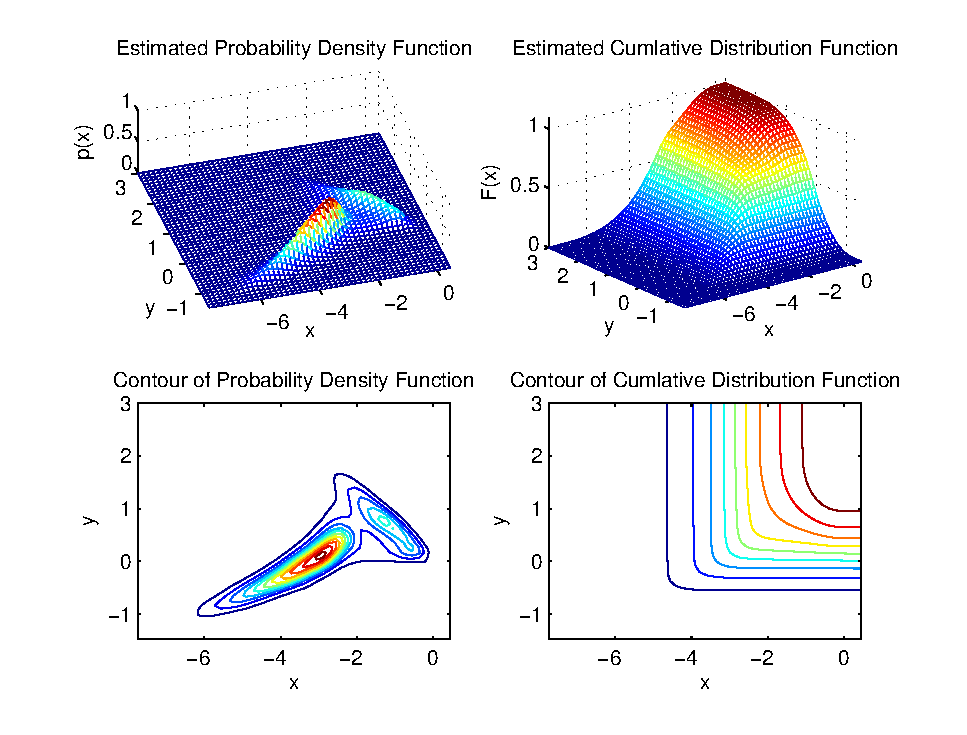
\includegraphics[width=\textwidth]{terrainDensity1vs2.eps}
                \caption{mixture }
                \label{fig:Mixture visualization in Terrain dataset component 1 vs 2}
        \end{subfigure}%

        \caption{Real mixture visualization in Terrain dataset component 1 vs 2 }\label{fig:animals}
\end{figure} 
\begin{figure}
        \centering
        \begin{subfigure}[b]{0.5\textwidth}
                \centering
                \includegraphics[width=\textwidth]{prior1.jpg}
                \caption{prior distribution }
                \label{fig:prior}
        \end{subfigure}%

        \caption{pictures of prior distribution }\label{fig:prior}
\end{figure}
{\bf B. Property of Dirichlet Distribution }  
For one single abundance fraction vector $s = (s_1,s_2,\dots, s_p)$. If we model it using Dirichlet distribution with parameter $\theta$. Then the model is the following:
\begin{equation}
\begin{aligned}
& \theta = (\theta_1,\theta_2,\dots,\theta_p), \theta_0=\sum_{i=1}^p \theta_i\\
& p_S(s|\theta ) = Dir(s|\theta) = \frac{\Gamma (\theta_0)}{\prod_{i=1}^p \Gamma(\theta_i) }\prod_{j=1}^p s_j^{\theta_j-1}\\
\end{aligned}
\end{equation}
The Dirichlet distribution is a distribution over the simplex $\sum_i s_i=1,s_i>=0$ So it automatically enforces the non negativity and sum-to-one constraint. To have a better geometric sense, let
\begin{equation}
\begin{aligned}
& \theta = (\theta_1,\theta_2,\dots,\theta_p) = \theta_0*(\beta_1,\beta_2,\dots,\beta_p); 
& \text{where } \theta_0=\sum_{i=1}^p \theta_i\\
\end{aligned}
\end{equation}
then  $(\beta_1,\beta_2,\dots,\beta_p)$ is the mean of the distribution,
and $ \theta_0$, which is called precision, represents how concentrate the data are. You can check 
the figure(?) and figure(?) to see how different parameter will effect the distribution. 
\begin{figure}
        \centering
        \begin{subfigure}[b]{0.3\textwidth}
                \centering
                \includegraphics[width=\textwidth]{(4,4,4).jpg}
                \caption{$\Gamma$ = (4,4,4), precision = 12 }
                \label{fig:gull}
        \end{subfigure}%
        ~ %add desired spacing between images, e. g. ~, \quad, \qquad etc. 
          %(or a blank line to force the subfigure onto a new line)
        \begin{subfigure}[b]{0.3\textwidth}
                \centering
                \includegraphics[width=\textwidth]{(10,10,10).jpg}
                \caption{$\Gamma$ = (10,10,10), precision = 30}
                \label{fig:tiger}
        \end{subfigure}
        ~ %add desired spacing between images, e. g. ~, \quad, \qquad etc. 
          %(or a blank line to force the subfigure onto a new line)
        \begin{subfigure}[b]{0.3\textwidth}
                \centering
                \includegraphics[width=\textwidth]{(2,2,2).jpg}
                \caption{$\Gamma$ = (0.2,0.2,0.2),precision = 0.6}
                \label{fig:mouse}
        \end{subfigure}
        \caption{Pictures of different precision}\label{fig:animals}
        \centering
        \begin{subfigure}[b]{0.3\textwidth}
                \centering
                \includegraphics[width=\textwidth]{(15,2,2).jpg}
                \caption{$\Gamma$ = (15,2,2) }
                \label{fig:gull}
        \end{subfigure}%
        ~ %add desired spacing between images, e. g. ~, \quad, \qquad etc. 
          %(or a blank line to force the subfigure onto a new line)
        \begin{subfigure}[b]{0.3\textwidth}
                \centering
                \includegraphics[width=\textwidth]{(15,25,2).jpg}
                \caption{$\Gamma$ = (15,25,2)}
                \label{fig:tiger}
        \end{subfigure}
        ~ %add desired spacing between images, e. g. ~, \quad, \qquad etc. 
          %(or a blank line to force the subfigure onto a new line)
        \begin{subfigure}[b]{0.3\textwidth}
                \centering
                \includegraphics[width=\textwidth]{(15,25,0).jpg}
                \caption{$\Gamma$ = (15,25,0.2)}
                \label{fig:mouse}
        \end{subfigure}
        \caption{Pictures of sparse presence component }\label{fig:animals}
\end{figure}
{\bf C.Model Abundance Using Single Dirchlet Distribution}  
Let us assume that $W = A^{-1}$ exists. Then, we have $S = WX$. Let us first consider use one single Dirichlet distribution to model the abundance. The parameters can be estimate from the likelihood function
\begin{equation}
\begin{aligned}
& L(W,\theta) = \log p_X(X | W,\theta) \\
&  =\sum_{i=1}^N \log p_X(x^{(i)} | W,\theta)\\
&  =\sum_{i=1}^N \log p_S(s^{(i)} | \theta)+N\log(\det|W|)\\
&  = N \log \Gamma(\sum_k \theta_k) - N \sum_k \log \Gamma(\theta_k) +  N \sum_k (\theta_k-1) \log \bar{s_k}+ N\log(\det|W|)\\
& \text{where}    \log \bar{s_k}  = \frac{1}{N} \sum_{i=1}^{N} \log s_{k}^{(i)}       \\
\end{aligned}
\end{equation}
So the optimization problem formed is the following: 
\begin{equation}
\begin{aligned}
& \underset{\theta,W}{\text{max}} \log \Gamma(\sum_k \theta_k) -  \sum_k \log \Gamma(\theta_k) +  \sum_k (\theta_k-1) \log \bar{(Wx)_k}+ \log(\det|W|)  \\
& \text{subject to}  (WX)_{i,j}\geq 0,\sum_i (WX)_{i,j} = 1\\
& \text{where}    \log \bar{(Wx)_k}  = \frac{1}{N} \sum_{i=1}^{N} \log (Wx^{(i)})_{k}    \\
\end{aligned}
\end{equation}

When $W$ is fixed, we can first calculate $S$ by $S=WX$, then the objective function over $\theta$  will be 
\begin{equation}
\begin{aligned}
\underset{\theta}{\text{max}} \log \Gamma(\sum_k \theta_k) -  \sum_k \log \Gamma(\theta_k) + \sum_k (\theta_k-1) \log \bar{s_k} \\
\end{aligned}
\end{equation}

Take derivative with respect to $\theta$ and set the gradient equal to $0$, we can get the following $p$ equations. 
\begin{equation}
\begin{aligned}
\log \bar{s_k} = \Phi(\theta_k) - \Phi(\sum_k \theta_k)\\
\text{where }\log \bar{s_k}  = \frac{1}{N} \sum_{i=1}^{N} \log s_{k}^{(i)}\\
\end{aligned}
\end{equation}
Here the function $\Phi(x)$ is the derivative for $ \log \Gamma(x)$. It behaves like a nature log function. since its derivative is decreasing, we can easily show that the objective function is convex with respect to $\theta$. On Nasci's paper, he provided a update method for $\theta_k$ by 
\begin{equation}
\begin{aligned}
\theta_k^{(t+1)} =\Phi^{-1} ( \Phi(\sum_k \theta_k^{(t)}) +\log \bar{s_k}^{(t)} )\\
\end{aligned}
\end{equation}
\begin{figure}
        \centering
        \begin{subfigure}[b]{0.5\textwidth}
                \centering
                \includegraphics[width=\textwidth]{Psi.jpg}
                \caption{$\Psi$ function }
                \label{fig:psi}
        \end{subfigure}%

        \caption{Pictures of $\Psi$ function }\label{fig:animals}
\end{figure}
This is essentially a fix-point method. Nasci's paper did not provide an initial guess and no proof for convergence. 
I give a good initial guess using the 1st and 2nd statistics of $S$ and the proof for convergence is in the Appendix. 
Since:
\begin{equation}
\begin{aligned}
E(s_{k}) = \frac{\theta_k}{\sum_k \theta_k}\\
E(s_{k}^2) = \frac{\theta_k(1+\theta_k)}{\sum_k \theta_k(1+\sum_k \theta_k)}
\end{aligned}
\end{equation}
We can show that 
\begin{equation}
\begin{aligned}
\theta_k = \frac{E(s_{k}) ^2-E(s_{k}) E(s_{k}^2) }{E(s_{k}^2) - E(s_{k}) ^2}
\end{aligned}
\end{equation}
This is a good initial guess for the parameters $\theta_k$.
\par But if we only use one Dirichlet density, it will have single mode. The mixture of Dirichlet density will allow one to model multi-mode densities. Then, the abundance fraction density has the following expression 
\begin{equation}
p_S(S|\theta ) = \sum_{q=1}^k \epsilon _qDir(S|\Theta _q) 
\end{equation}
For fixed $W$ , a EM algorithm is employed to estimate the parameters in the mixture of Dirichlet density.  The formulas  are similar except for assigning fuzzy membership weight for each data. \\
\setcounter{chapter}{4}
\setcounter{equation}{0} %-1
{\bf 4. Data Set and Experiment Results }
1. Real Data Visualization
\par As we mentioned above, the density of the abundance plays important role in deciding which model to choose. Below is a set of data visualization, to show how the real data are. 
 \begin{figure}
        \centering
        \begin{subfigure}[b]{1.0\textwidth}
                \centering
                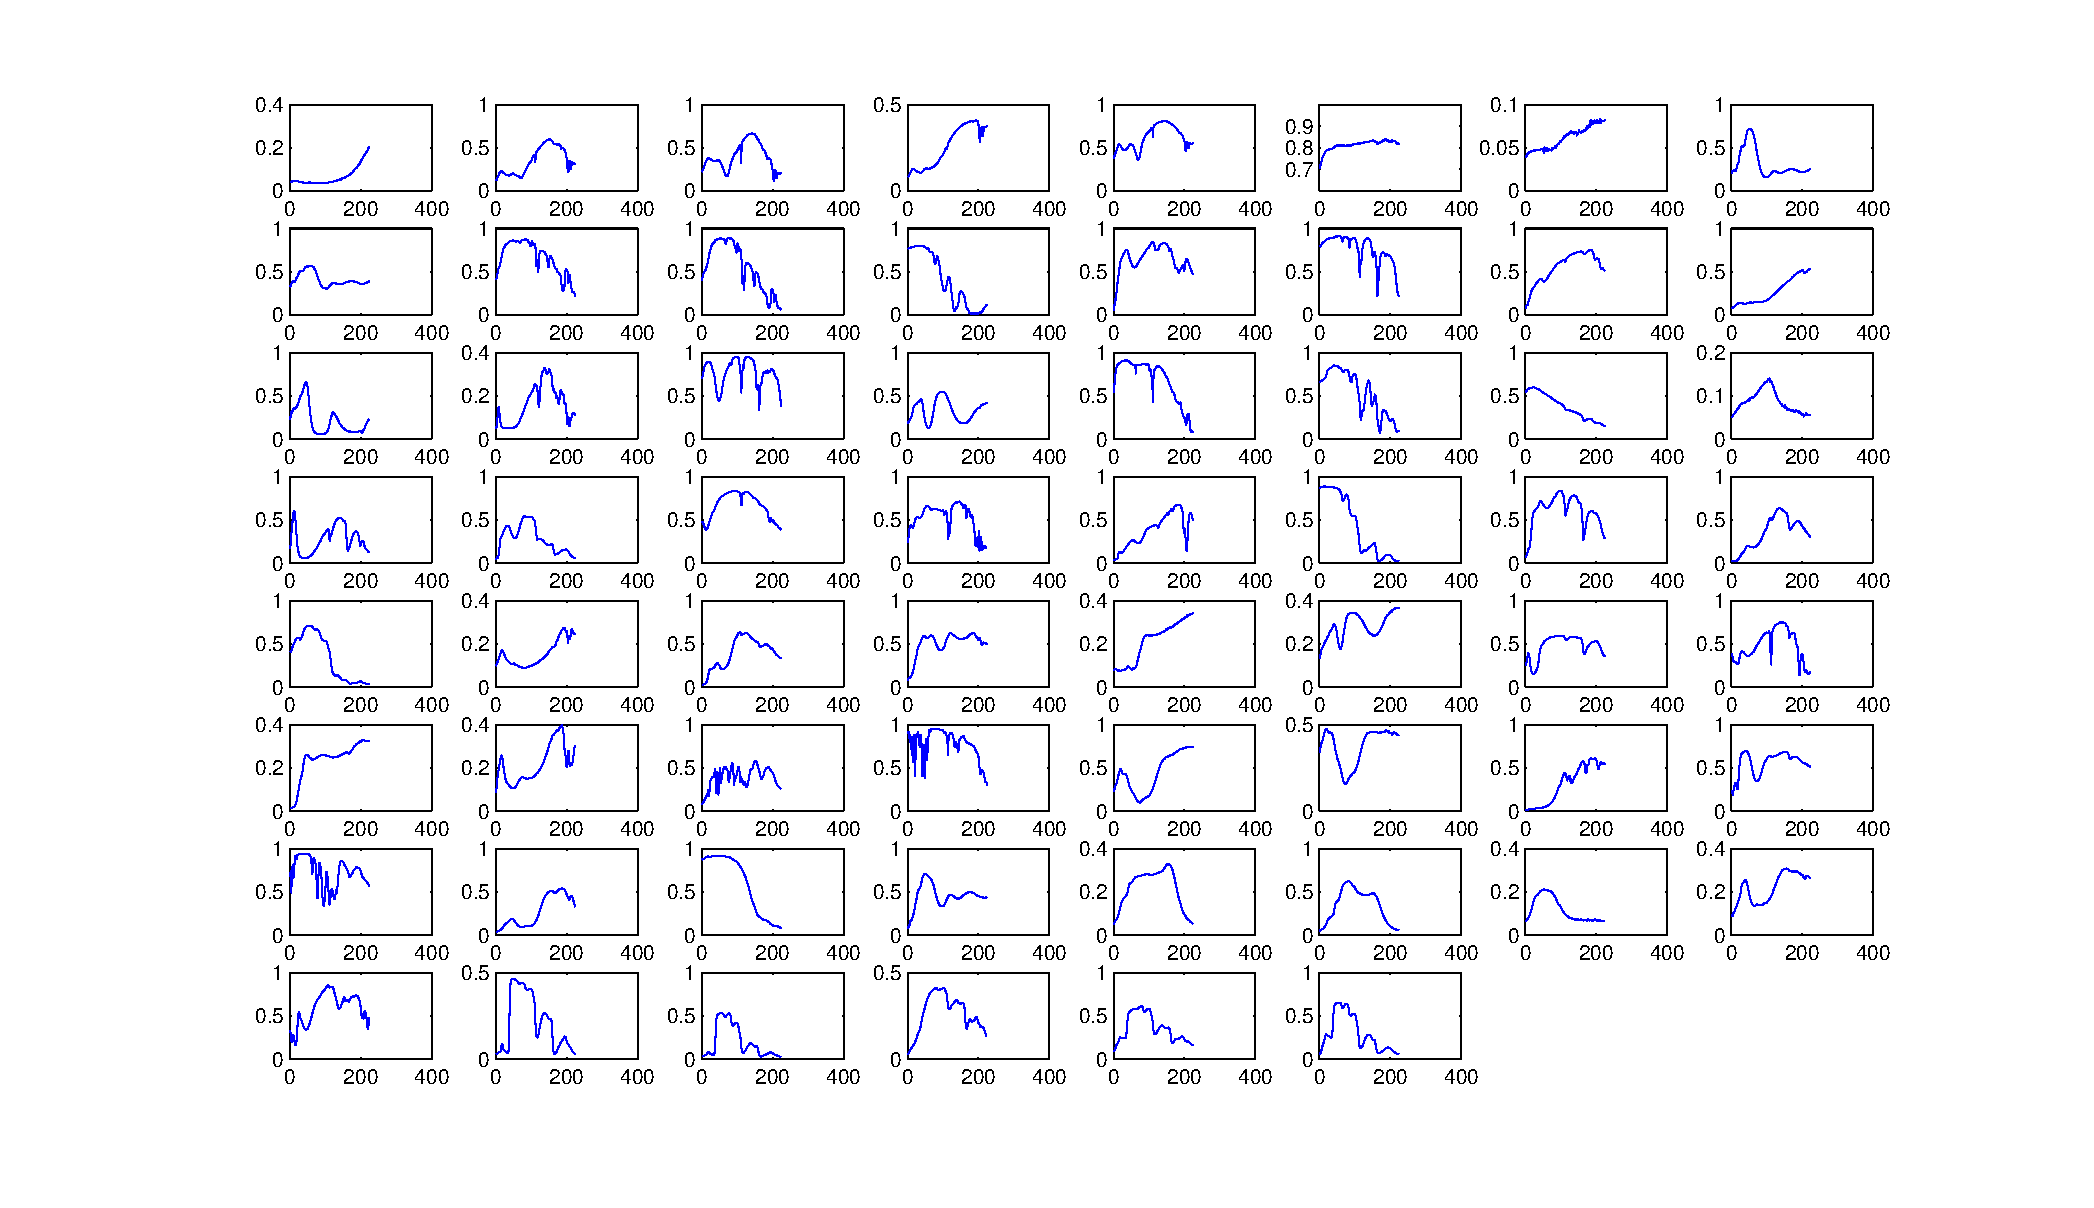
\includegraphics[width=\textwidth]{endmembers.eps}
                \caption{endmembers }
                \label{fig:endmembers visualization in USGS dataset}
        \end{subfigure}%

        \caption{endmembers visualization in USGS dataset }\label{fig:animals}
\end{figure}
 \begin{figure}
        \centering
        \begin{subfigure}[b]{1.0\textwidth}
                \centering
                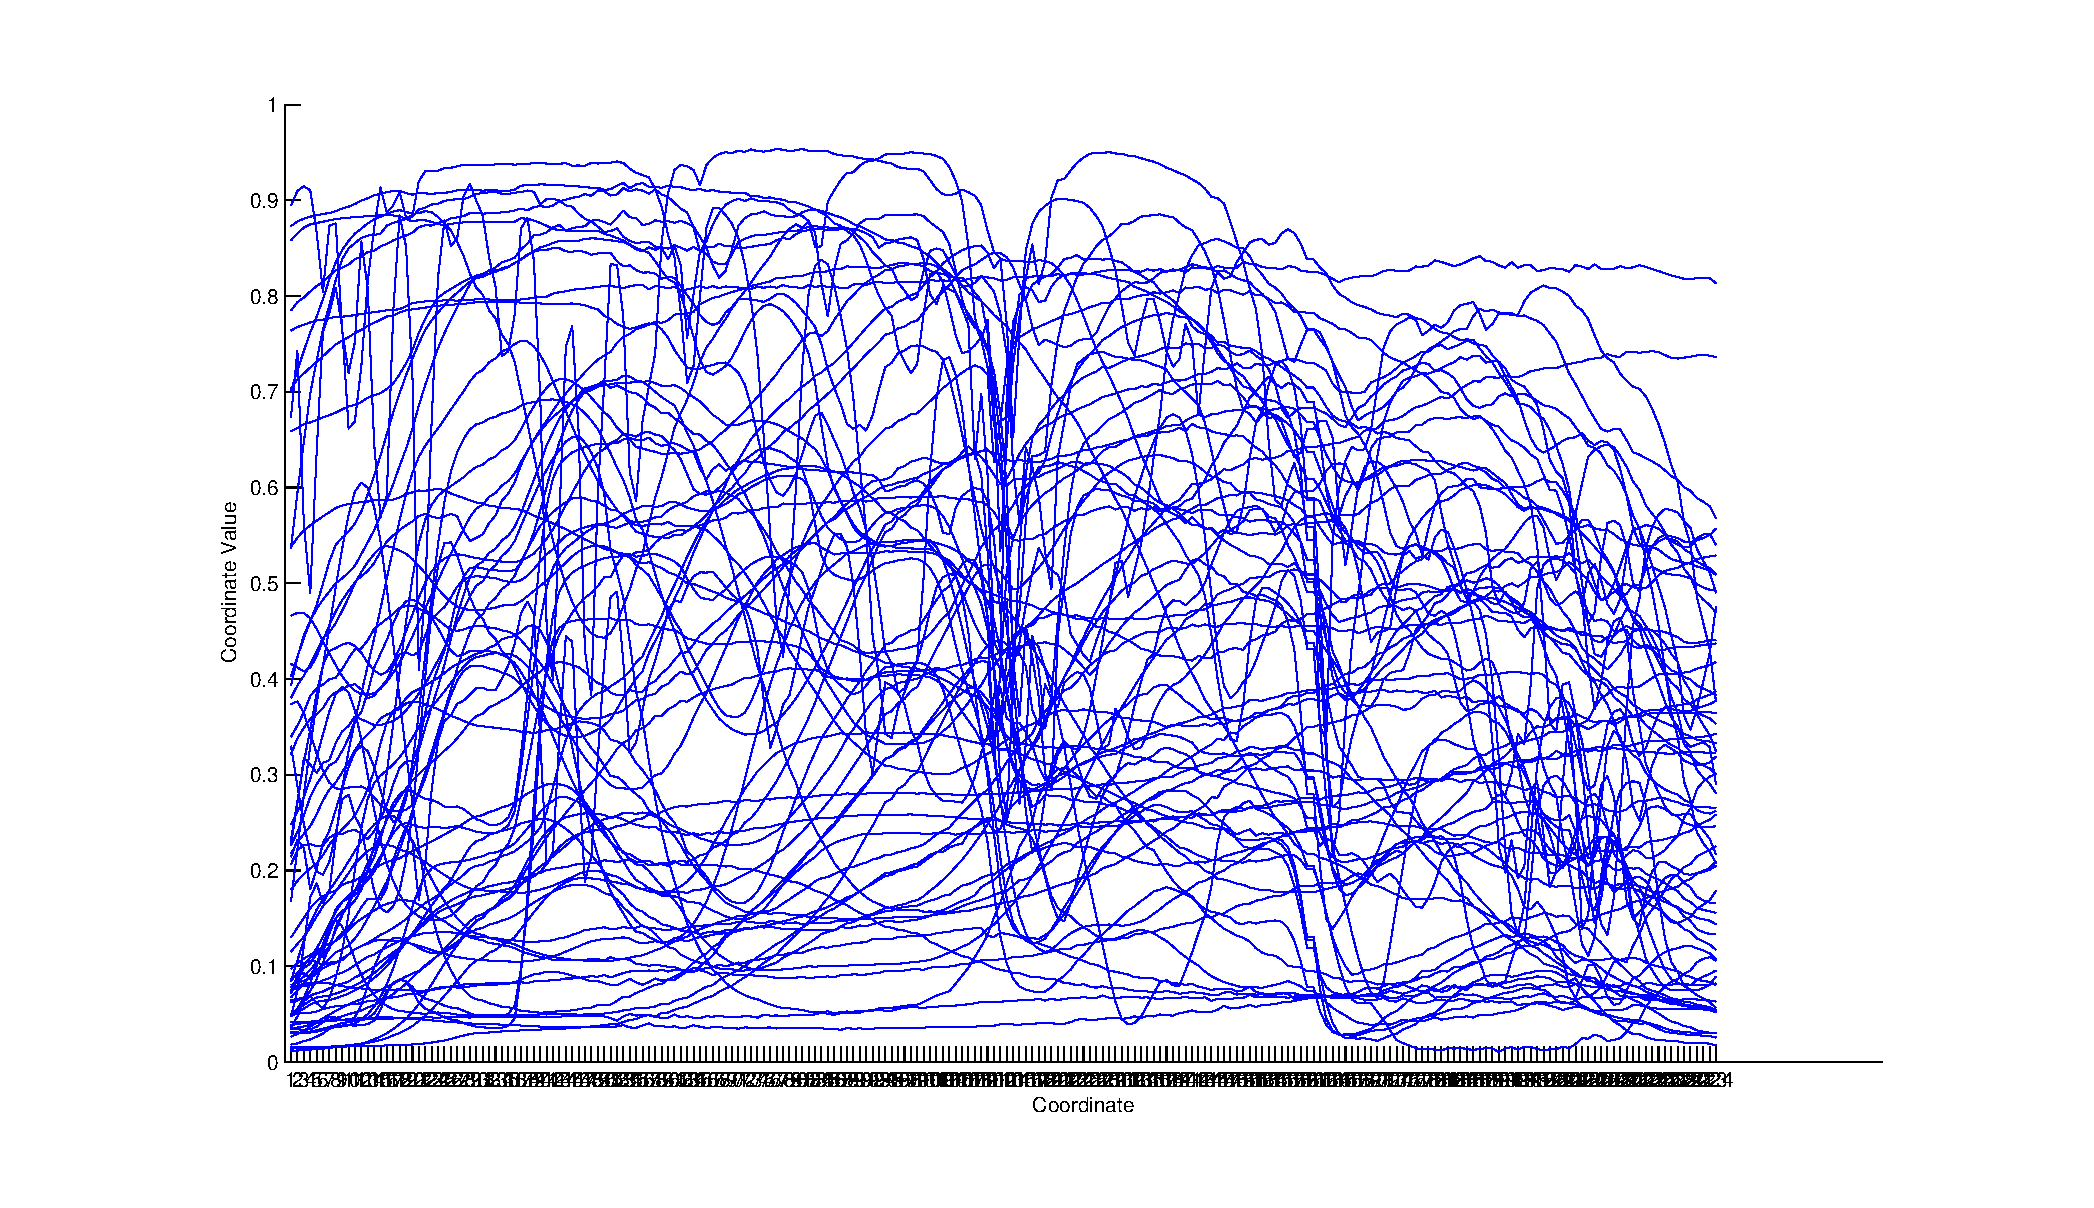
\includegraphics[width=\textwidth]{endmembers2.eps}
                \caption{endmembers }
                \label{fig:endmembers visualization in USGS dataset}
        \end{subfigure}%

        \caption{endmembers visualization in USGS dataset }\label{fig:animals}
\end{figure}

The first mixture dataset is Terrain dataset. it contains HYDICE sensor imagery We first use hysime algorithm to reduce the dimension of the data from  166*153500 to 24*153500. It can be consider as 153500 data points on the 24 dimensional space. We would be interested in the density of these data points to verify the model for abundance. 
 \begin{figure}
        \centering
        \begin{subfigure}[b]{1.0\textwidth}
                \centering
                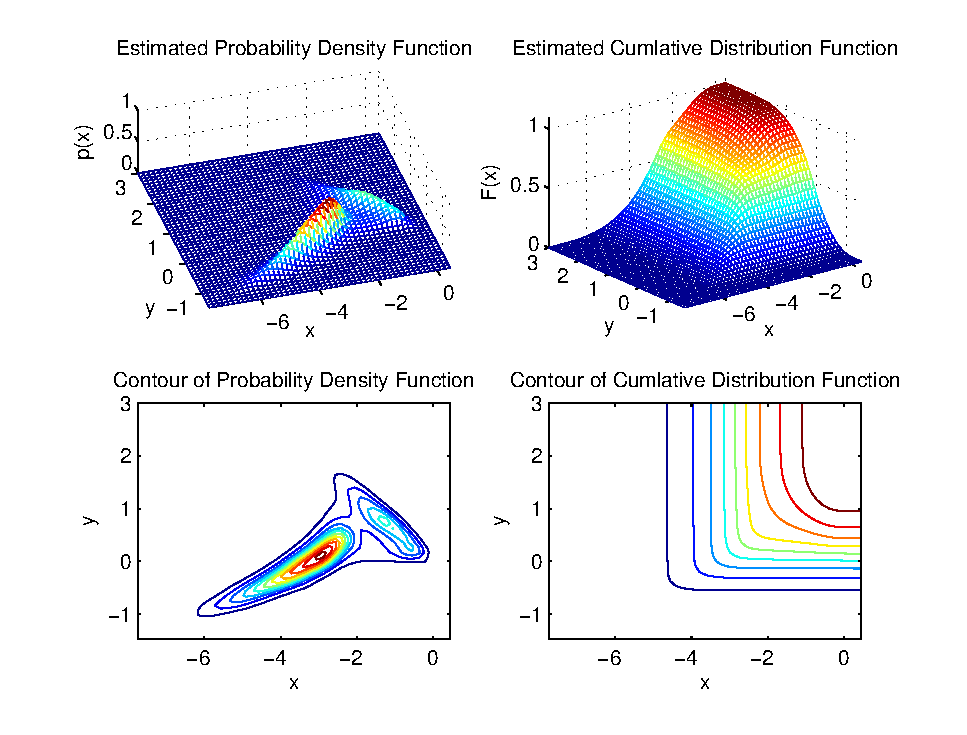
\includegraphics[width=\textwidth]{terrainDensity1vs2.eps}
                \caption{mixture }
                \label{fig:Mixture visualization in Terrain dataset component 1 vs 2}
        \end{subfigure}%

        \caption{Mixture visualization in Terrain dataset component 1 vs 2 }\label{fig:animals}
\end{figure}
 \begin{figure}
        \centering
        \begin{subfigure}[b]{1.0\textwidth}
                \centering
                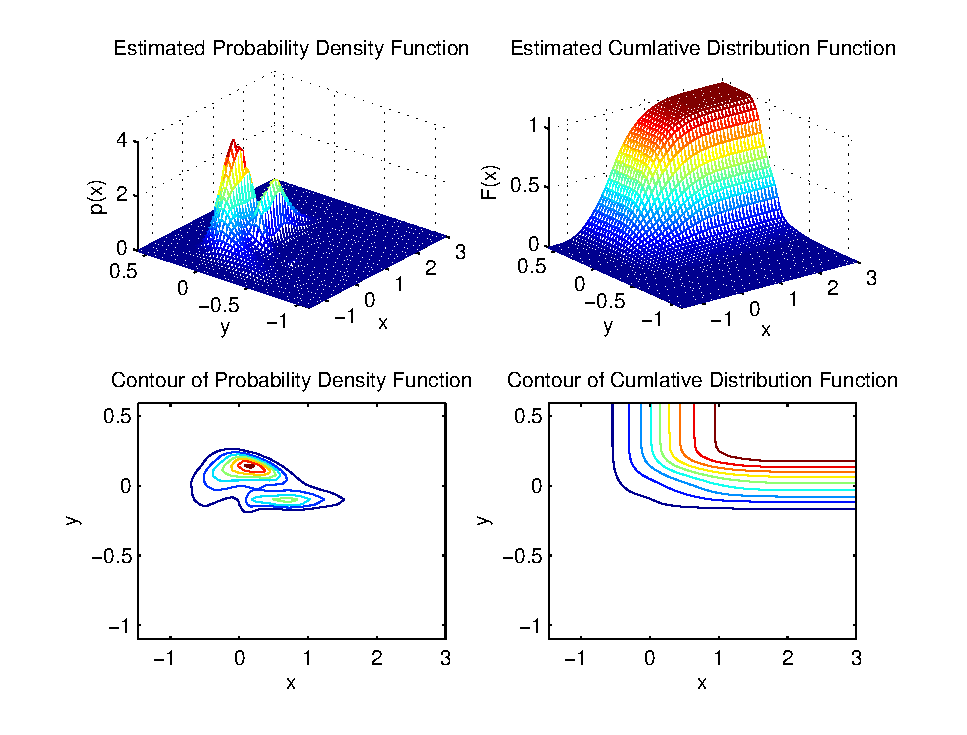
\includegraphics[width=\textwidth]{terrainDensity2vs3.eps}
                \caption{mixture }
                \label{fig:Mixture visualization in Terrain dataset component 2 vs 3}
        \end{subfigure}%

        \caption{Mixture visualization in Terrain dataset component 2 vs 3}\label{fig:animals}
\end{figure}

2. Synthetic Data Experiments 
The mixing matrix is random sampled from USGS dataset. The abundance are sampled from Dirichlet distribution with parameter $\theta$ and mixing weights $\epsilon$ \\ . First, we compare the performance of Minimum Volume Algorithm and Dirichlet Component Based Algorithm. 
Experiment 1: 
\par $\theta =\begin{pmatrix} 
18 & 6 &  3\\ 
 13& 14 & 4 \\ 
 4 & 5 & 16 
\end{pmatrix}$, $\epsilon = [0.4,0.4,0.2]$ \\
\begin{figure}
        \centering
        \begin{subfigure}[b]{1\textwidth}
                \centering
                \includegraphics[width=\textwidth]{r11.jpg}
                \caption{Experiment 1 }
                \label{fig:psi}
        \end{subfigure}%

        \caption{Experiment 1 }\label{fig:animals}
\end{figure}
We can see that when precision is large, here 
 The Dirichlet Algorithm significantly improve  Minimum Volume Algorithm. 
  \begin{figure}
        \centering
        \begin{subfigure}[b]{1\textwidth}
                \centering
                \includegraphics[width=\textwidth]{r12.jpg}
                \caption{Experiment 1 }
                \label{fig:psi}
        \end{subfigure}%

        \caption{Experiment 1 }\label{fig:animals}
\end{figure}
Experiment 2: \\
\par $\theta =\begin{pmatrix} 
0.5 & 0.3 & 8\\ 
 0.4& 0.9 & 2.2 \\ 
 15 & 14 & 0.7 
\end{pmatrix}$, $\epsilon = [0.2,0.3,0.5]$ \\
We can see for the case that some of the $\theta$ parameters are $\le 1$, The minimum volume algorithm tend to give good results since most of the data are on the facet of the simplex. 
\begin{figure}
        \centering
        \begin{subfigure}[b]{1\textwidth}
                \centering
                \includegraphics[width=\textwidth]{r21.jpg}
                \caption{Experiment 2 }
                \label{fig:psi}
        \end{subfigure}%

        \caption{Experiment 2 }\label{fig:animals}
\end{figure}\\
\setcounter{chapter}{5}
\setcounter{equation}{0} %-1
\noindent {\bf 4. Future Work}

\setcounter{chapter}{5}
\setcounter{equation}{0} %-1
\begin{thebibliography} {99}
\end{thebibliography}
\vskip .65cm
\noindent
first author affiliation
\vskip 2pt
\noindent
E-mail: (first author email)
\vskip 2pt
\noindent
second author affiliation
\vskip 2pt
\noindent
E-mail: (second author email)
\vskip .3cm
%\centerline{(Received xxx 200?; accepted xxx 200?)}\par
\end{document}